
% This document is for the Group Meeting Agenda.  The Agenda should
% be distributed to each member (and other invitees) and to the TA
% prior to the meeting (hopefully the day before) so that each member
% will have adequate time to prepare for the meeting.  The best way
% to accomplish the distribution of the agenda is to email the LaTeX
% file to all members and TA.
%
%\documentstyle[fullpage]{article}
\documentclass[a4paper,12pt]{article}
\usepackage{fullpage}
\usepackage{cite}
\usepackage{url}
\usepackage{xcolor}
\usepackage{setspace}
\usepackage[version=4]{mhchem}
\usepackage{upgreek}
\usepackage[margin=0.75in]{geometry}
% For figure:
\usepackage{graphicx}
\usepackage{float}
% For table:
\usepackage{makecell}
\makeatletter
% we use \prefix@<level> only if it is defined
\renewcommand{\@seccntformat}[1]{%
  \ifcsname prefix@#1\endcsname
    \csname prefix@#1\endcsname
  \else
    \csname the#1\endcsname\quad
  \fi}
% define \prefix@section
\newcommand\prefix@section{}
\makeatother
\begin{document}

%
% This section gives the general information about the meeting such
% as the title, who it was called by, when and where the meeting
% will take place, what type of meeting it is (planning, design,
% problem-solving, decision-making, etc.), and of course who is
% invited to attend.
%

\pagestyle{fancyplain}
\fancyhf{}
\lhead{ \fancyplain{}{BIOL 4020 – Vertebrate Biodiversity - Amphibians}}
%\chead{ \fancyplain{}{}}
\rhead{ \fancyplain{}{Fall 2020}}
%\rfoot{\fancyplain{}{page \thepage\ of \pageref{LastPage}}}
\fancyfoot[RO, LE] {page \thepage\ of \pageref{LastPage}}
\thispagestyle{plain}

\begin{figure}[H]
\centering
  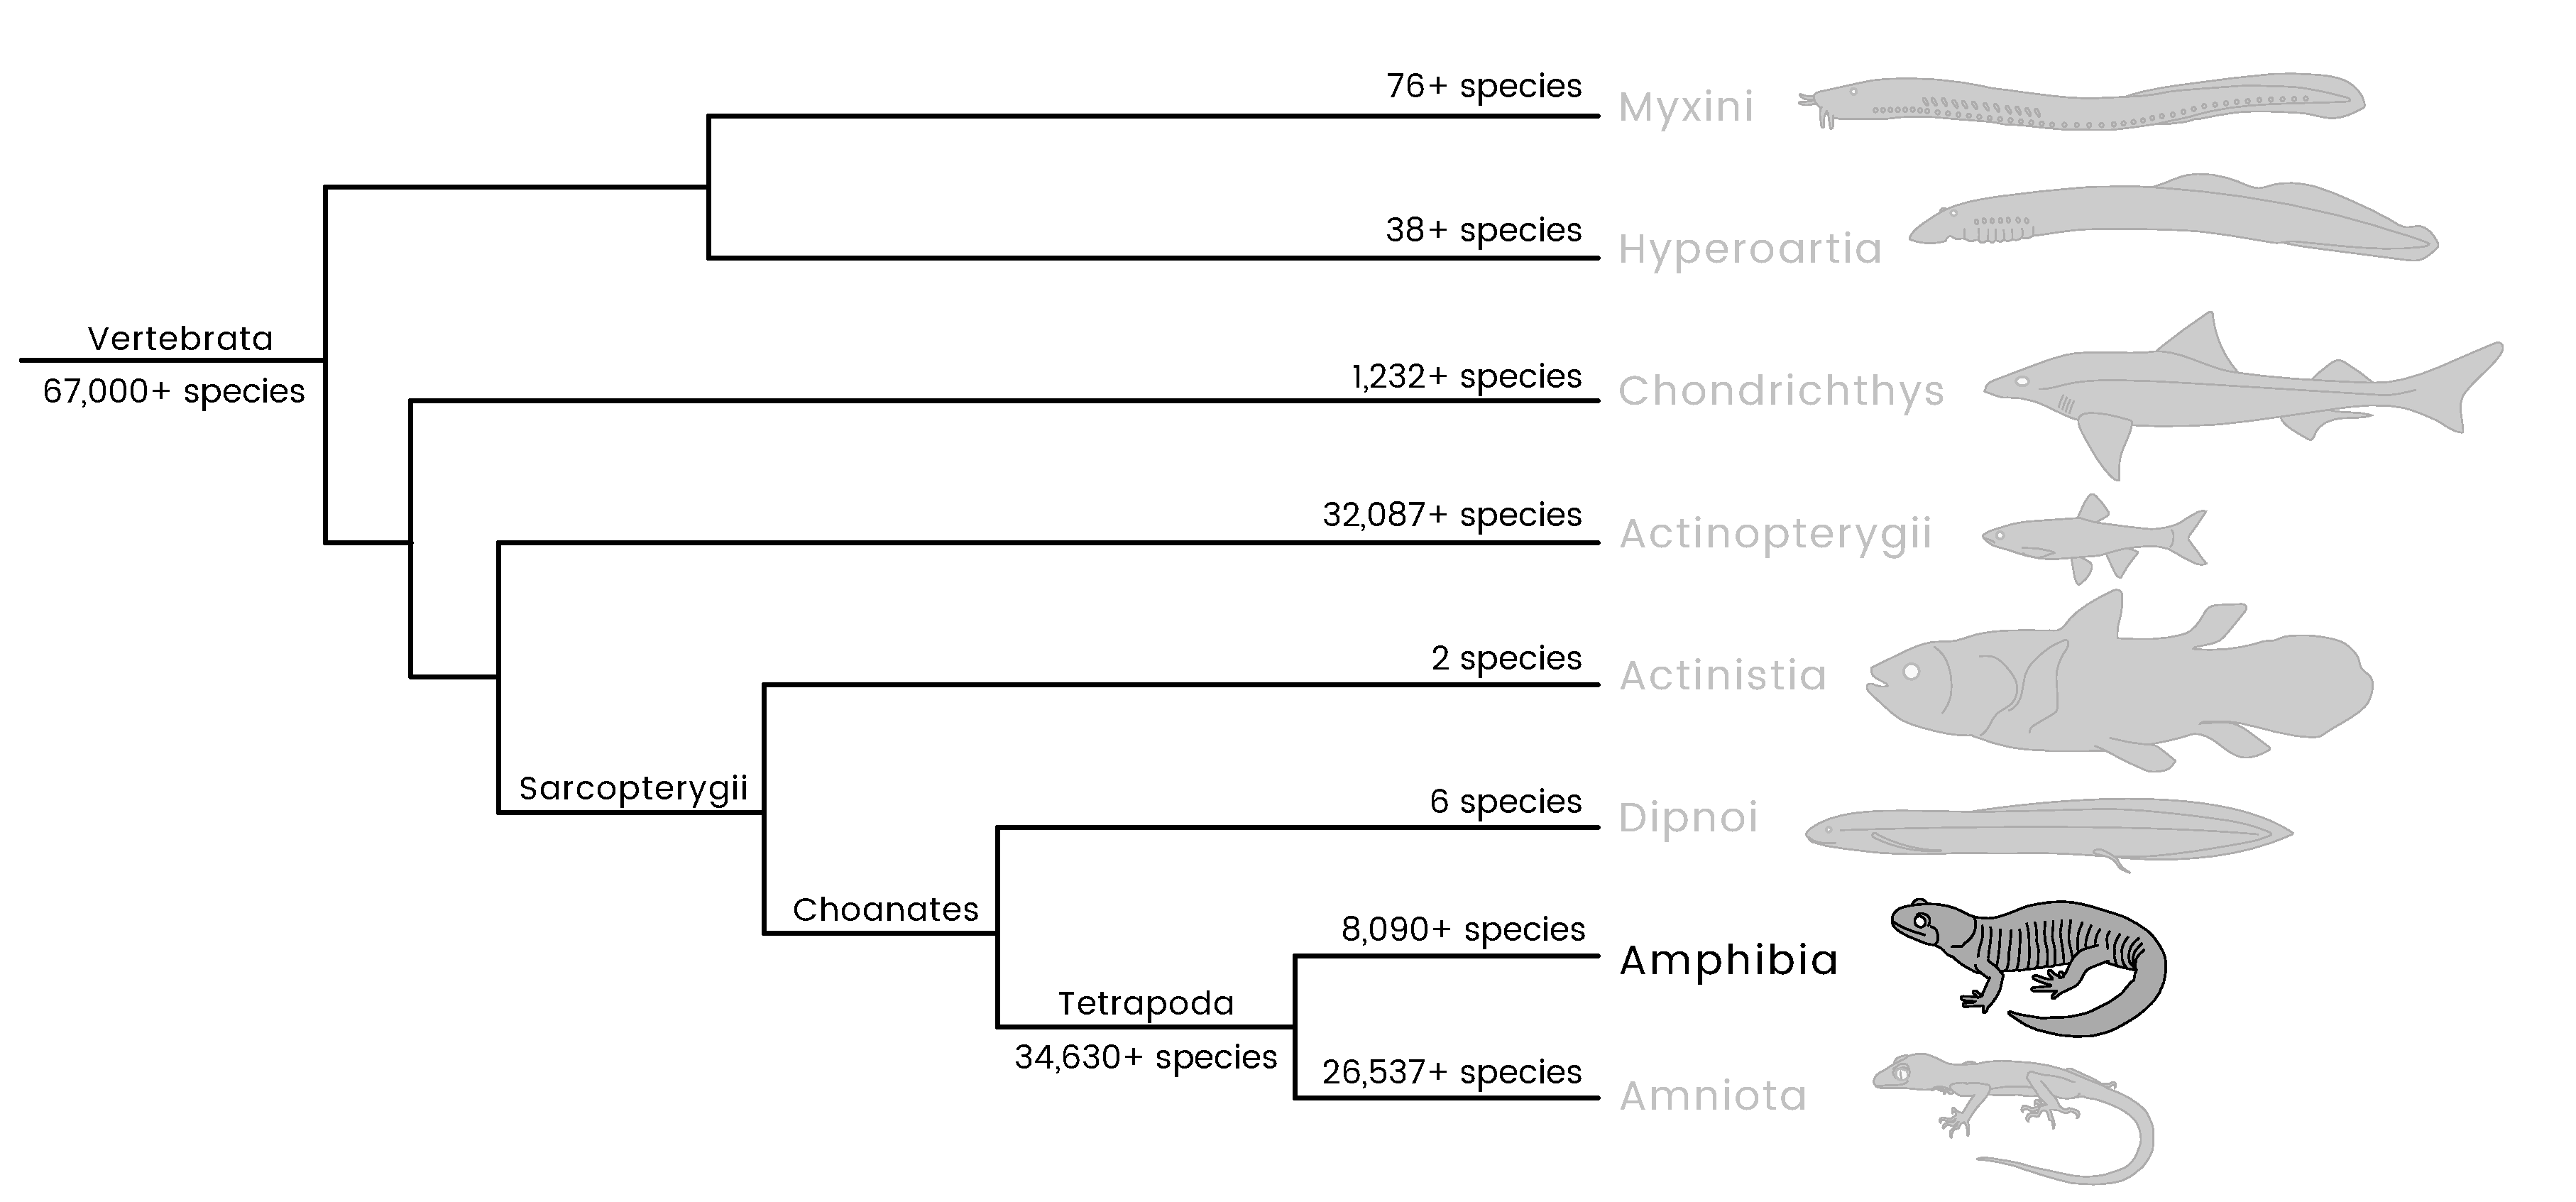
\includegraphics[scale=0.4]{Vertebrata_amphib_tre.pdf}
  \caption{Amphibian placement within Vertebrata}
  \label{fig:Vertebrates2}
\end{figure}

\begin{figure}[H]
\centering
  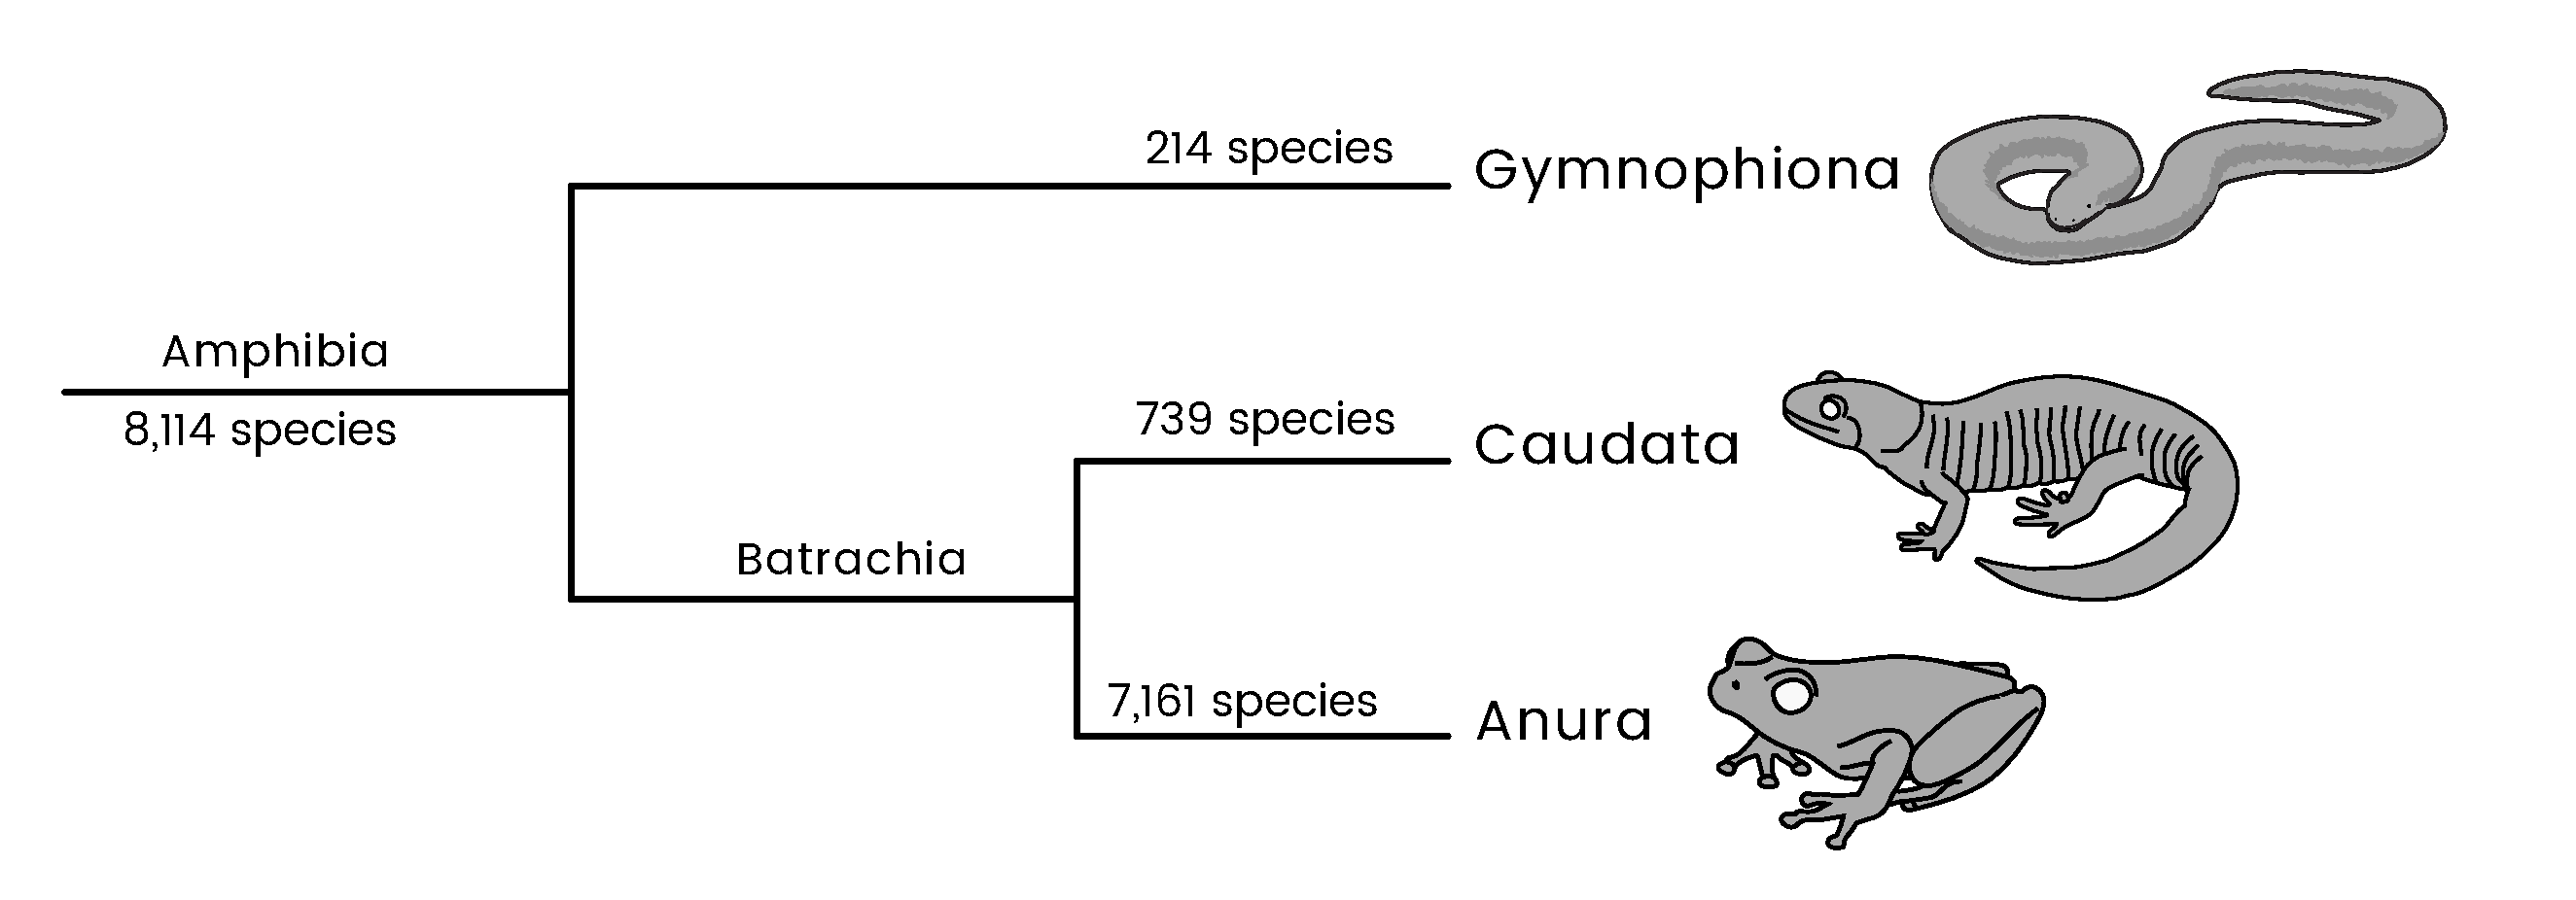
\includegraphics[scale=0.4]{Amphibia_tre.pdf}
  \caption{Amphibian Relationships}
  \label{fig:Amphibia}
\end{figure}

\begin{figure}[h]
\centering
  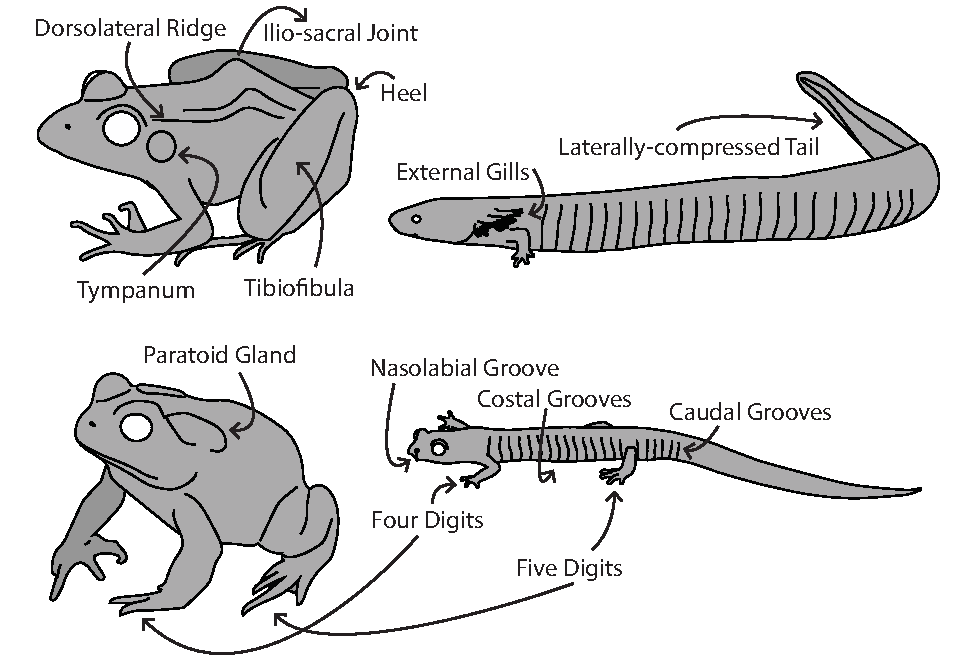
\includegraphics{AmphibianAnatomy.pdf}
  \caption{Amphibian anatomical terms to know}
  \label{fig:Anura}
\end{figure}

\section*{Focal taxonomic groups} ($\star$ groups you need to be able to photo ID and place in a phylogeny. $\mathsection$ denotes species for which you need to audio ID calls.)
\begin{description}
\item{\underline{{\LARGE{Gymnophiona}}}}
(Caecilians) No limbs, cylindrical body, tail short or absent, cloaca towards end of body, strong skull with pointed snout, pair of tentacles between eyes and mouth (olfactory), bodies distinctly segmented by annuli (each segment contains a single vertebra)

\begin{figure}[H]
\centering
  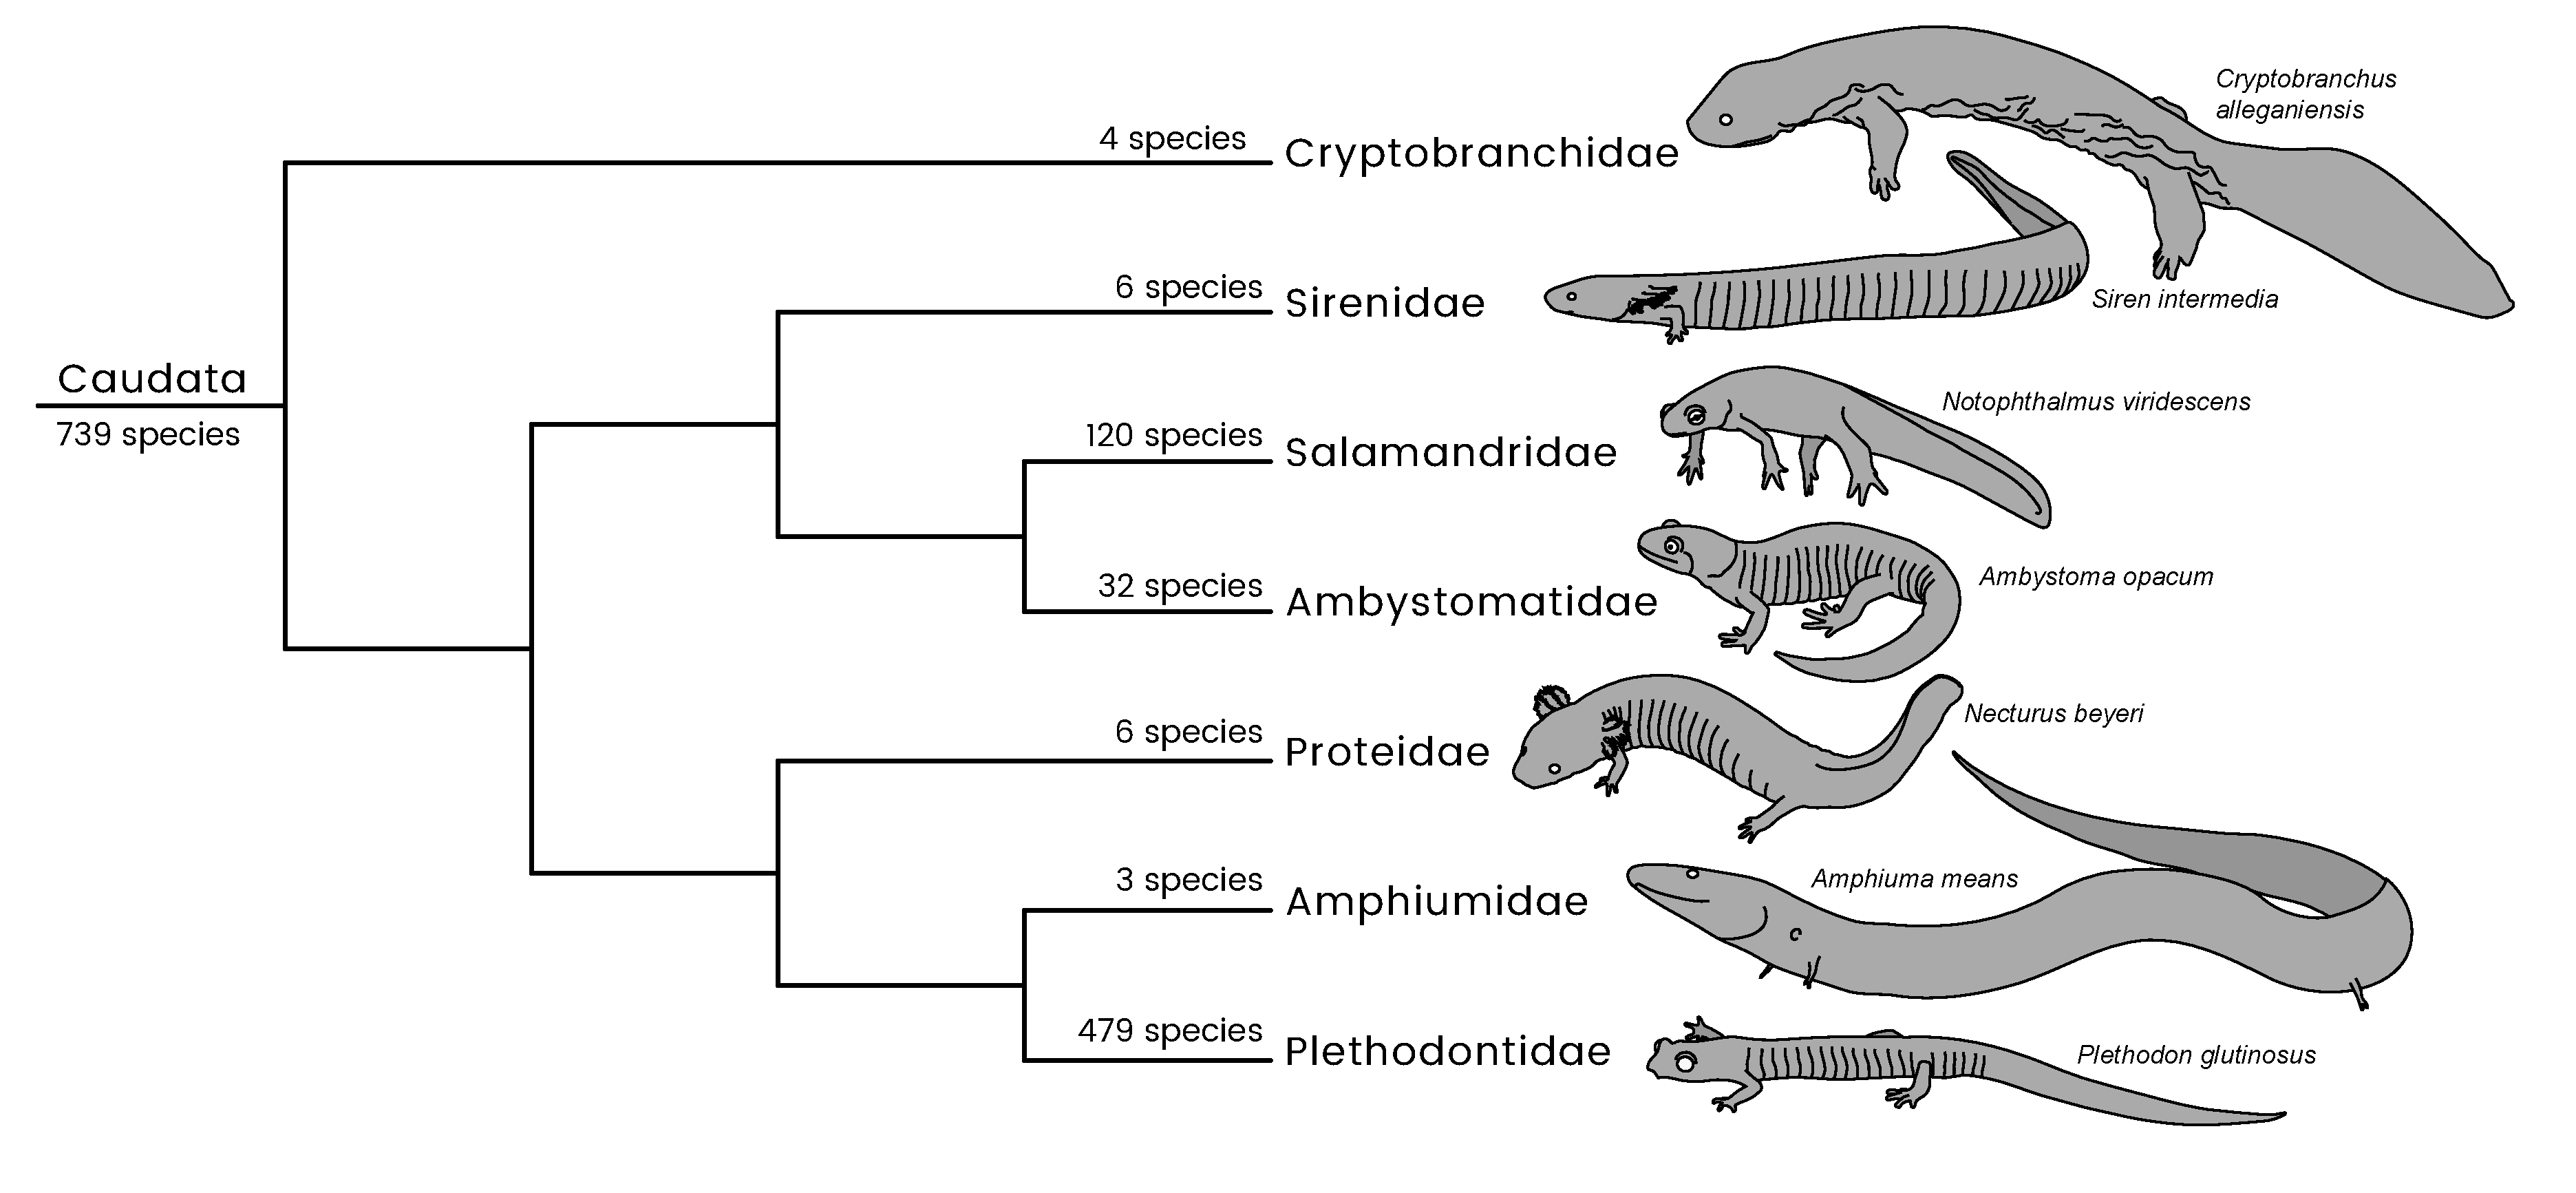
\includegraphics[scale=0.4]{Caudata_tre.pdf}
  \caption{Caudata Relationships (abbreviated)}
  \label{fig:Caudata}
\end{figure}

\item{\underline{{\LARGE{Caudata}}}}
(Salamanders) tailed, body not globular
\begin{itemize}
  \item{\textbf{family CHRYPTOBRANCHIDAE} (giant salamanders)$\star$} \\ largest living salamanders, stout bodies, four short and well-developed limbs, laterally compressed tail, single pair of gill slits
  \begin{itemize}
    \item{\textbf{\textit{Chryptobranchus alleganiensis}} (American hellbender)$\star$} \\ Flat head, fringe of skin along sides of body, external gill openings but no visible gills, reduced eyes
  \end{itemize}
  \item{\textbf{family SIRENIDAE} (sirens)} \\ No hind limbs, external gills
  \begin{itemize}
    \item{\textbf{\textit{Siren intermedia}} (lesser siren)$\star$} \\ Less than 36 costal grooves
  \end{itemize}  
  \item{\textbf{family SALAMANDRIDAE} (newts and European salamanders)} \\ Four limbs, no gill openings, no nasolabial groove, ridge down middorsum, no costal grooves (or costal grooves above ribs), rough skin
  \begin{itemize}
    \item{\textbf{\textit{Notophthalmus viridescens}$\star$} (Eastern newt)} \\ Adult stage: olive / yellow ground color, spotted (red spots in reproductively active males); Eft stage: red or orange ground color with red spots
  \end{itemize}
  \item{\textbf{family AMBYSTOMATIDAE} (mole salamanders)} \\ Costal grooves present, dorsum round and lacking ridge, no nasolabial grooves, heavy bodied, heavy tailed, lack gills and gill slits and have moveable eyelids
  \begin{itemize}
    \item{\textbf{\textit{Ambystoma opacum}} (marbled salamander)$\star$} \\ black ground color with white/silvery crossbands on dorsum (some of which are ocassionally broken- more pronounced in males)
    \item{\textbf{\textit{Ambystoma maculatum}} (spotted salamander)$\star$} \\ black ground color with orange/yellow dorsal spots or blotches
    \item{\textbf{\textit{Ambystoma mexicanum}} (axolotl)} \\ larval traits retained (no moveable eyelinds, external gills), model organism
  \end{itemize}
  \item{\textbf{family PROTEIDAE} (water dogs)$\star$} \\ External gills, four well-developed limbs, moderately robust body, laterally compressed tails
  \begin{itemize}
    \item{\textbf{\textit{Necturus beyeri}} (Gulf Coast waterdog)} \\ cylindrical body, four toes on front and hind limbs, spotted body (light spotting in adults)
  \end{itemize}
  \item{\textbf{family AMPHIUMIDAE} (congo eels)$\star$} \\ External gill slits, four reduced limbs (with 3 or fewer toes)
  \begin{itemize}
    \item{\textbf{\textit{Amphiuma means}} (two-toed amphiuma)} \\ 2 toes on each limb
  \end{itemize}
  \item{\textbf{family PLETHODONTIDAE} (lungless salamanders)$\star$} \\ Nasolabial grooves, four well-developed limbs with 4-5 toes, no ridge down mid-dorsum, slim body
  \begin{itemize}
    \item{\textbf{genus\textit{ Desmognathus}} (dusky salamanders)$\star$} \\ face with light stripe from eye to angle of jaw
    \item{\textbf{\textit{Eurycea cirrigera}} (two-lined salamander)} \\ yellowish to orange-brown dorsum with dark dorsolateral stripe from snout to near tail tip
    \item{\textbf{\textit{Plethodon glutinosus}$\star$} (Southern slimy slamander)} \\ elongate body, ground color brown to black with light spots or flecks
    \item{\textbf{\textit{Pseudotriton ruber}} (red salamander)} \\ dull to bright red with black flecks
  \end{itemize}
\end{itemize}

\begin{figure}[h]
\centering
  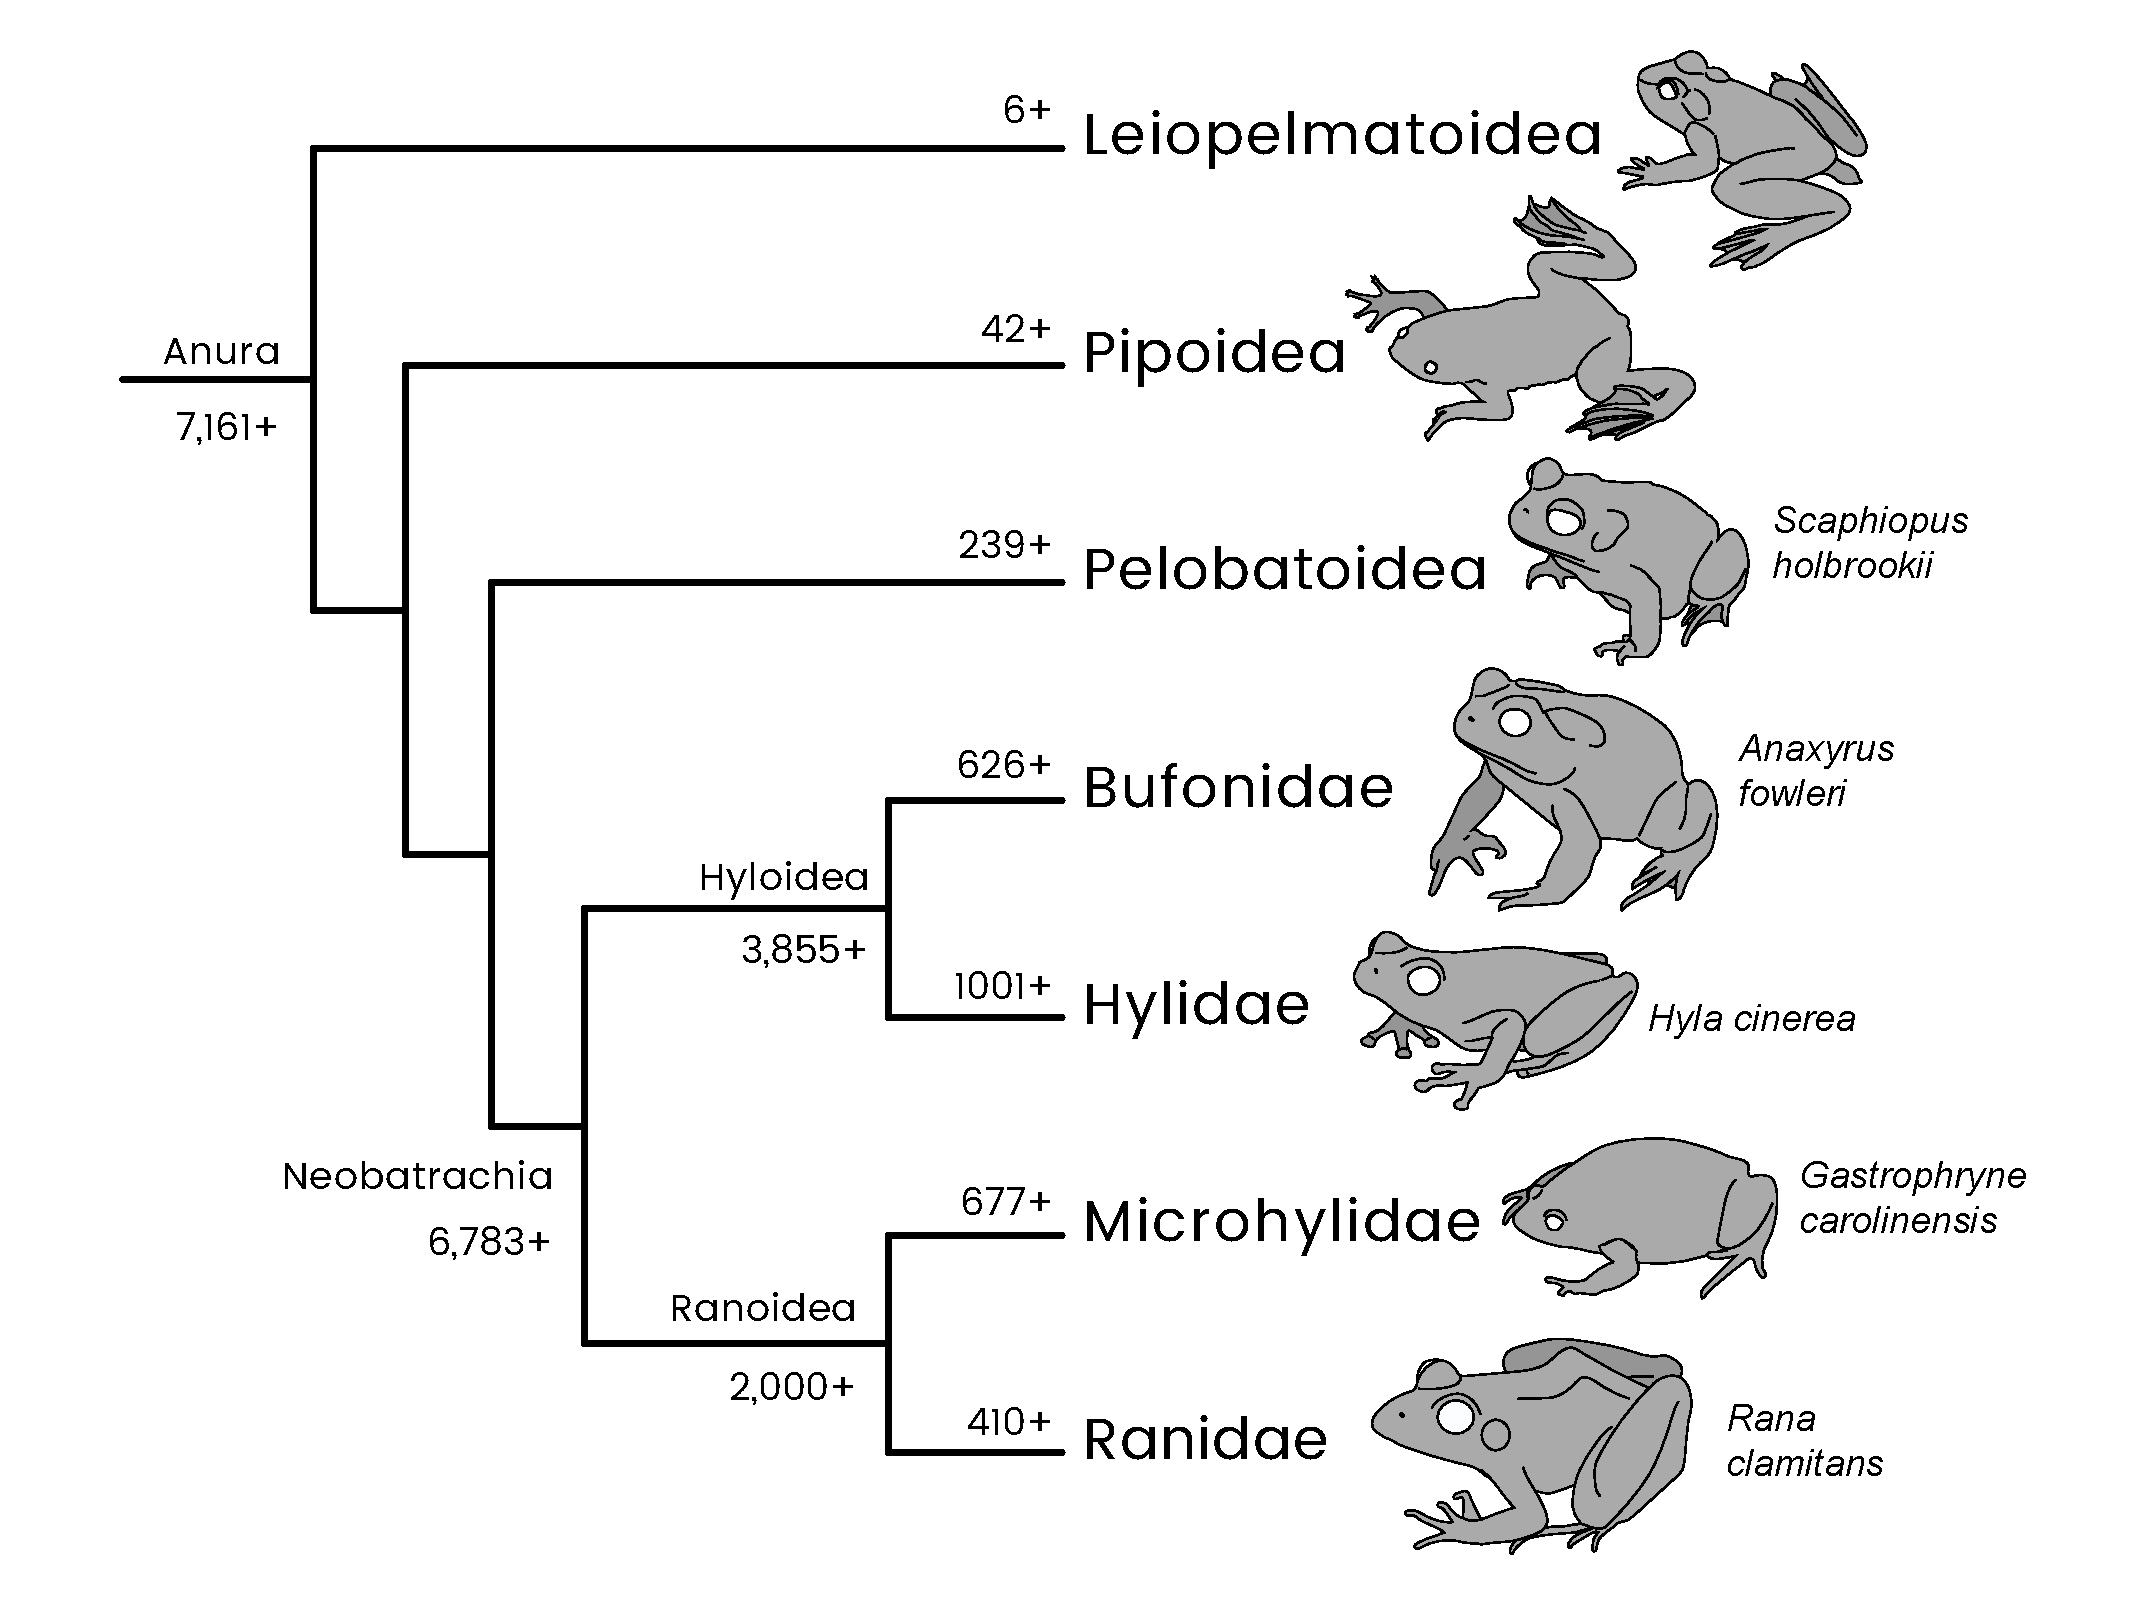
\includegraphics[scale=0.4]{Anura_tre.pdf}
  \caption{Anura Relationships (abbreviated)}
  \label{fig:Anura}
\end{figure}

\item{\underline{{\LARGE{Anura}}}}
(Frogs) tailless with globular body
\begin{itemize}
  \item{\textbf{Leiopelmatoidea}}
  \begin{itemize}
    \item{\textbf{genus\textit{Ascaphus}} (Tailed frog)} \\ modification of cloaca and tail muscles produces intromittent or copulatory organ in males
  \end{itemize}
  \item{\textbf{Pipoidea}}
  \begin{itemize}
    \item{\textbf{family PIPIDAE}} \\ dorsoventrally depresed bodies and large muscular hindlimbs with webbed feet
    \begin{itemize}
      \item{\textbf{\textit{Pipa pipa}} (Suriname toad)} \\ extreme dorsoventral compression with squared head, females carry eggs and developing tadpoles on their backs
      \item{\textbf{\textit{Xenopus laevis}} (African clawed frog)} \\ somewhat egg-shaped body, fully webbed toes, three toes on each foot have conspicuous black claws
    \end{itemize}
  \end{itemize}
  \item{\textbf{Pelobatoidea}}
  \begin{itemize}
    \item{\textbf{family SCAPHIOPODIDAE} (spadefoot toads)} \\ squat body, warty (but soft) skin, large keratinous-edged crescent-shaped tubercle on outer edge of eat hind foot, webbed hind feet
    \begin{itemize}
      \item{\textbf{\textit{Scaphiopus holbrooki}} (Eastern spadefoot)$\star$ $\mathsection$} \\ vertically elliptical pupils, absent or indistinct paratoid glands
    \end{itemize}
  \end{itemize}
  \item{\textbf{family BUFONIDAE} (true toads)$\star$} \\ squat body, short hind limbs, enlarged toepads, 2 spade-like tubercles on hind feet, round pupil, pronounced paratoid glands, skin dry and warty, throats of males usually dark
  \begin{itemize}
      \item{\textbf{\textit{Anaxyrus fowleri}} (Fowler's toad)$\star$ $\mathsection$} \\ Paratoid gland touches postorbital ridge, three or more warts in each of largest spots, common "backyard" toad
  \end{itemize}
  \item{\textbf{familiy HYLIDAE} (tree frogs and allies)} \\ long hind limbs, usually enlarged toepads
  \begin{itemize}
    \item{\textbf{genus\textit{Acris}} (cricket frogs)$\star$ $\mathsection$} \\ Rear of thigh with one or two longitudinal stripes, front of snout with lighvertical lines, hind webbing half-way along fourth toe
    \item{\textbf{genus\textit{Hyla}}} \\ Hind webbing half-way along fourth toe, greatly expanded toe disks
    \begin{itemize}
      \item{\textbf{\textit{Hyla cinerea}} (green tree frog)$\star$ $\mathsection$} \\ bright green with white/yellow lateral racing stripe
      \item{\textbf{\textit{Hyla avivoca}} (bird-voiced tree frog)$\star$ $\mathsection$} \\ coloration variable (gray to green), back of thigh pale yellow to greenskin of dorsum smooth to slightly papillate or pustulate
    \end{itemize}
    \item{\textbf{genus\textit{Pseudacris}} (chorus frogs)} \\ No webbing on hind toes, tips of digits expanded
    \begin{itemize}
      \item{\textbf{\textit{Pseudacris crucifer}} (spring peeper)$\star$ $\mathsection$} \\ distinct x pattern on dorsum, small toe pads
    \end{itemize}
  \end{itemize}
  \item{\textbf{familiy RANIDAE} (true frogs)$\star$} \\ No toe pads, extensive toe webbing, expanded tympanic membrane
  \begin{itemize}
    \item{\textbf{\textit{Rana catesbeianus}} (American bullfrog)$\star$ $\mathsection$} \\ Tympanic membrane larger than eye, no dorsal-lateral ridge (ridge ends at tympanum), largest frog in North America
    \item{\textbf{\textit{Rana sphenocephalus}} (Southern leopard frog)$\star$ $\mathsection$} \\ Dorsal-lateral ridge reaches groin, rounded dark spots on dorsum, pointed snout
    \item{\textbf{\textit{Rana clamitans}} (bronze frog)$\star$ $\mathsection$} \\ Dorsal-lateral ridge doesn't reach groin, tympanum same size as eye
  \end{itemize}
  \item{\textbf{familiy MICROHYLIDAE} (narrow-mouth frogs)$\star$} \\ supradigital scutes. Members of this family have lipophilic alkaloids (derived from ant diet) that can be highly toxic$\star$note: this family isn't on the tree, but is nested within \textbf{Hyloidea}
  \begin{itemize}
    \item{\textbf{\textit{Gastrophryne carolinensis}} (narrow-mouth toad)$\star$ $\mathsection$} \\ Small, tiny head with pointed snout, no webbing between digits
  \end{itemize}\end{itemize}
\end{description}

\end{document}
